%%%%%%%%%%%%%%%%%%%%%%%%%%%%%%  IEEEsample.tex
%%%%%%%%%%%%%%%%%%%%%%%%%%%%%%%%%%%%%%%%%
%%%%%%%%%%%%%%%%%%%%%%%    More information: see the header of IEEEtran.sty
%%%%%%%%%%%%%%%%%%%%%%%
%%%%%%%%%%%%%%%%%%%%%%%%%%%%%%%%%%%%%%%%%%%%%%%%%%%%%%%%%%%%%%%%%%%%%%%%%%%%%%%%
%%%%

\documentclass{llncs}

%\usepackage[ruled]{algorithm}
\usepackage{algorithmic}

\renewcommand{\algorithmicrequire}{\textbf{Input:}}
\renewcommand{\algorithmicensure}{\textbf{Output:}}

\usepackage{helvet}
\usepackage{enumerate}
\usepackage{amsmath}
\usepackage{amsfonts}
\usepackage{graphicx}
\usepackage{multirow}
\usepackage{subfig}
\usepackage[ruled]{algorithm2e}
%\RequirePackage{algorithmic}
%\RequirePackage{algorithm}
\usepackage{blkarray}
\usepackage{cases}

\renewcommand{\algorithmiccomment}[1]{/* #1 */}

\input{epsf}
\def\BibTeX{{\rm B\kern-.05em{\sc i\kern-.025em b}\kern-.08em1
    T\kern-.1667em\lower.7ex\hbox{E}\kern-.125emX}}

%\newtheorem{Definition}{definition}[section]
%\newtheorem{example}{Example}
%\newtheorem{Lemma}{Lemma}

% New command for the table notes.
\def\tabnote#1{{\small{#1}}}

% New command for the line spacing.
\newcommand{\ls}[1]
    {\dimen0=\fontdimen6\the\font
     \lineskip=#1\dimen0
     \advance\lineskip.5\fontdimen5\the\font
     \advance\lineskip-\dimen0
     \lineskiplimit=.9\lineskip
     \baselineskip=\lineskip
     \advance\baselineskip\dimen0
     \normallineskip\lineskip
     \normallineskiplimit\lineskiplimit
     \normalbaselineskip\baselineskip
     \ignorespaces
    }

\newcommand{\beq}{\begin{equation}}
\newcommand{\eeq}{\end{equation}}
\newcommand{\ov}{\overline}
%\newcommand{\ov}{\bar}
\newcommand{\xor}{\bigoplus}
%%
%\newtheorem{algorithm}{Algorithm}[section]


%%%%%%%%
%From Irina
\usepackage[english]{babel}

\newtheorem{defn}{Definition}[section]
%\usepackage{datetime}
\newtheorem{thm}[defn]{Theorem} % definition numbers are dependent on
% theorem
% %
\newtheorem{prop}[defn]{Proposition} % definition numbers are dependent on
\newtheorem{dem}[defn]{Proof} % definition numbers are dependent on
              % numbers
\newtheorem{exemp}{Example}[defn]
\newtheorem{lema}{\bf Lemma}[defn]

%%%%%
%% \newtheorem{Algorithm}{Algorithm}[section]
%% \newtheorem{Definition}{Definition}[section]
%% \newtheorem{Example}{Example}[section]
%% \newtheorem{Proposition}{Proposition}[section]
%% \newtheorem{Lemma}{Lemma}[section]
%% \newtheorem{Theorem}{Theorem}[section]
%% \newtheorem{Corollary}{Corollary}[section]
%% \newtheorem{Problem}{Problem}[section]
%% \newtheorem{Conjecture}{Conjecture}[section]
%% \newtheorem{Result}{Result}[section]
%%%%%

\newtheorem{Problem}{Problem}

\def\opn#1#2{\def#1{\operatorname{#2}}} % to make operators

\opn\Ker{Ker} \opn\Coker{Coker}  \opn\Hom{Hom} \opn\Im{Im}
\opn\End{End} \opn\Aut{Aut} \opn\defect{def} \opn\ord{ord}
\opn\id{id} \opn\dim{dim} \opn\det{det} \opn\tr{tr} \opn\grad{grad} \opn\lcm{LCM}
\opn\min{min} \opn\max{max} \opn\det{det}
%\def\Frob{{\mathcal F}}
\opn\Span{Span}   \opn\rang{rang}  \opn\id{id} \opn\dim{dim} \opn\ad{ad} \opn\tr{tr} \opn\ker{ker}
\opn\GL{GL} \opn\SL{SL} \opn\mod{mod} \opn\diag{diag}
\opn\min{min} \opn\sgn{sgn} \opn\ini{in_<}  \opn\Mon{Mon} \opn\LC{LC_<}
\opn\LT{LT_<}
\opn\s{supp}  


\newcommand{\Z}{{\mathbb{Z}}}
\newcommand{\F}{{\mathbb{F}}}
\newcommand{\Fc}{\overline{\mathbb{F}}}
\newcommand{\R}{{\mathbb{F}[x_1,\dots,x_d]}}
\newcommand{\bi}{\begin{itemize}}
\newcommand{\ei}{\end{itemize}}
%%%%%%%%
\begin{document}

\title{Finding Infeasible Cores of a Set of Polynomials using the Gr\"obner Basis Algorithm}

\author{Xiaojun Sun\inst{1} \and Irina Ilioaea\inst{2} \and Priyank Kalla\inst{1} \and Florian Enescu\inst{2}}
\institute{ 
Electrical and Computer Engineering, University of Utah, Salt Lake City UT, USA \\
\email{\{xiaojuns, kalla\}@ece.utah.edu}
\and
Mathematics and Statistics, Georgia State University, Atlanta GA, USA\\
\email{iilioaea1@student.gsu.edu, fenescu@gsu.edu}
}

\maketitle

\thispagestyle{plain}
\pagestyle{plain}

\begin{center}{\bf ABSTRACT}\end{center}
Formal verification of hardware designs has become an essential
component of the overall system design flow. The designs are generally
modeled as finite state machines, on which property and equivalence
checking problems are solved for verification. Reachability analysis
forms the core of these techniques. However, increasing
size and complexity of the circuits causes the state explosion
problem. Abstraction is key to tackle the scalability challenge.

This dissertation presents new techniques for word-level abstraction
with applications in sequential design verification. By bundling
together $k$ bit-level state-variables into one word-level constraint 
expression, the state-space is construed as solutions (variety) to
a set of polynomial constraints (ideal), modeled over the finite
(Galois) field of $2^k$ elements. Subsequently, techniques from
algebraic geometry -- notably, Gr\"obner basis theory and technology
-- are researched to perform reachability analysis and
verification of sequential circuits. This approach adds a ``word-level
dimension'' to state-space abstraction and verification to make the
process more efficient.

While algebraic geometry provides powerful abstraction and reasoning
capabilities, the algorithms exhibit high computational complexity. In
the dissertation, we show that by analyzing the constraints, it is
possible to obtain more insights about the polynomial ideals, which can be
exploited to overcome the complexity. Using our algorithm design and
implementations, we demonstrate how to perform reachability
analysis of finite-state machines purely at the word-level. Using this
concept, we perform scalable verification of sequential arithmetic
circuits. As contemporary approaches make use of resolution proofs and
unsatisfiable cores for state-space abstraction, we introduce the
algebraic geometry analog of unsatisfiable cores, and present
algorithms to extract and refine unsatisfiable cores of polynomial
ideals. Experiments are performed to demonstrate the efficacy of our
approaches. 

%\section{Introduction}

{\bf This is the dummy submission uploaded on Feb 21. The final paper will be uploaded on Feb 24, 2016.}


Let $F=\{f_1,f_2,\ldots,f_m\}$ be a set of $m$ polynomials in $\mathbb{F}_2[x_1,\ldots,x_n]$ and $I=(F)$ the ideal generated by the set $F$. Assume that our term order is LEX with $x_1>x_2>...>x_n$. Suppose that it is known that $V(I)=\emptyset$.
 
We can now apply the Buchberger's algorithm \cite{HH} to the system of generators $F$ of $I$.
 
Next, we will keep track of the S-polynomials that give non-zero remainder when divided by the system of generators of $I$ at that moment.
\begin{center}
$g_{ij}:= S(f_i,f_j)-\displaystyle\sum_{k=1}^l c_kf_k$,
\end{center}
where $0\neq c_k\in\mathbb{F}_2[x_1,\ldots,x_n]$ and $\{f_1,\ldots,f_l\}$ is the current system of generators of $I$.

For each non-zero $g_{ij}$, we will record the following data:
$$((g_{ij})(f_i,f_j)(h_{ij},h_{ji})| (f_1,\ldots,f_l),(c_1,\ldots,c_l))$$


 Note that here $g_{ij}$ denotes the remainder of the $S$-polynomial $S(f_i,f_j)$ modulo the current system of generators $f_1,\ldots,f_l$ of the ideal $I$ and we denote by 
$$h_{ij}:=\displaystyle\frac{\lcm(\ini(f_i),\ini(f_j))}{\LT(f_i)}, h_{ji}:=\displaystyle\frac{\lcm(\ini(f_i),\ini(f_j))}{\LT(f_j)}$$
the coefficients of $f_i$, respectively $f_j$ in the $S$-polynomial $S(f_i,f_j)$.


I recall that we have $$S(f_i,f_j)=\displaystyle\frac{\lcm(\ini(f_i),\ini(f_j))}{\LT(f_i)}f_i-\frac{\lcm(\ini(f_i),\ini(f_j))}{\LT(f_j)}f_j$$.

The last part contains the $f_i$'s that appear in the division process and the second parentheses has the corresponding coefficients.

 When we obtain $1$ as a remainder of a $S$-polynomial to the current system of generators, we stop.

As an output of the Buckberger's Algorithm, we can obtain not only the Gr\"obner bases, let's call it $\{g_1,\ldots,g_t\}$, but also a matrix $M$ such that
\begin{center}
\begin{align}
   \begin{bmatrix}
           g_{1} \\
           g_{2} \\
           \vdots \\
           g_{t}
         \end{bmatrix}
    &= M \begin{bmatrix}
           f_{1} \\
           f_{2} \\
           \vdots \\
           f_{m}
         \end{bmatrix}
  \end{align}

\end{center}
\begin{thm}
With the notations above, we have that a core for the system of generators $F$ of the ideal $I$ is given by the union of those $f_i$'s from $F$ that appear in the data recorded above and correspond to the nonzero entries in the matrix $M$. 
\end{thm}

\begin{proof}
In our case, $g_1=1$ and $t=1$, since the variety is empty, and hence the ideal is the unit ideal. Say $M= [a_1, \ldots, a_m]$. Then the output of the algorithm gives

$$1 = a_1f_1+\cdots + a_m f_m.$$ Clearly, if $a_i=0$ for some $i$ then $f_i$ does not appear in this equation and should not be included in the core.

\end{proof}


%
%

 Our next goal will be to describe an algorithm that allows us to compute a core of the ideal and the matrix $M$.

INITIAL DATA: $S_0=\{f_1,\ldots,f_m\}$ system of generators of the ideal $I$, monomial order $<$ on $\mathbb{F}_2[x_1,\ldots,x_n]$.

STEP 1: We start computing the S-polynomials of the system of generators $\{f_1,\ldots,f_m\}$ as in the Buchberger's algorithm \cite{HH}. After computing the first one, we divide it by the system of generators $S_0$. In this way, we will obtain the following expression
$$g_{i_1i_2}:= h_{i_1i_2}f_{i_1}-h_{i_2i_1}f_{i_2}-\displaystyle\sum_{k=1}^m c_kf_k$$

If the remainder $g_{i_1i_2}$ is non-zero, we will denote it by $f_{m+1}$ and we will add it to our initial system of generators. We will also record the data as follows
$$((f_{m+1}:=g_{i_1i_2})(f_{i_1},f_{i_2})(h_{i_1i_2},h_{i_2i_1})| (f_1,\ldots,f_m),(c_1,\ldots,c_m))$$ 
Then we will consider $S_1:=\{f_1,\ldots,f_m,f_{m+1}\}$ to be the new system of generators of $I$.

STEP s:  If $S_s:=\{f_1,\ldots,f_{s}\}$ is the current system of generators of $I$ and we have the following relation for $f_s$
$$f_s=g_{ij}=h_{ij}f_i-h_{ji}f_j-\displaystyle\sum_{k=1}^{s-1} a_kf_k$$

and the recorded data 
$$((f_{s}:=g_{ij})(f_{i},f_{j})(h_{ij},h_{ji})| (f_1,\ldots,f_{s-1}),(a_1,\ldots,a_{s-1}))$$

We will compute the next S-polynomial which gives a non-zero remainder when divided by our current system of generators $S_s$
$$f_{s+1}=g_{pq}=h_{pq}f_p-h_{qp}f_q-\displaystyle\sum_{k=1}^s b_kf_k$$
  
By substituting $f_s$ in the expression of $f_{s+1}$ we get 
$$f_{s+1}= h_{pq}f_p-h_{qp}f_q-\displaystyle\sum_{k=1}^{s-1} b_kf_k-b_s(h_{ij}f_i-h_{ji}f_j-\displaystyle\sum_{k=1}^{s-1} a_kf_k)$$
$$= h_{pq}f_p-h_{qp}f_q-\displaystyle\sum_{k=1}^{s-1} b_kf_k-b_sh_{ij}f_i+b_sh_{ji}f_j+\displaystyle\sum_{k=1}^{s-1} b_sa_kf_k$$
$$= h_{pq}f_p-h_{qp}f_q-b_sh_{ij}f_i+b_sh_{ji}f_j+\displaystyle\sum_{k=1}^{s-1} (b_sa_k-b_k)f_k$$

 Next, we will record the data for $f_{s+1}$
$$((f_{s+1}:=g_{pq})(f_{p},f_{q})(h_{pq},h_{qp})| (f_1,\ldots,f_{s-1},f_i,f_j),(b_sa_1-b_1,\ldots,b_sa_{s-1}-b_{s-1},b_sh_{ij},b_sh_{ji}))$$


The algorithm will stop when we will obtain the last non-zero remainder $f_l=1$. After using the previous relations, we will have the following
$$1=f_l=\displaystyle\sum_{k=1}^{m} d_kf_k$$
OUTPUT:
the core of the system of generators $S_0$ is $\{f_k: k\in\overline{1,m}, d_k\neq 0\}$
        
the matrix with the coefficients  $$M=(d_1,\ldots,d_k)$$.
	\begin{exemp}
Consider the following set of polynomials:
\begin{center}
$f_1: abc + ab + ac + bc + a + b + c + 1$
\end{center}
\begin{center}
$f_2: b$
\end{center}
\begin{center}
$f_3: ac$
\end{center}
\begin{center}
$f_4: ac + a$
\end{center}
\begin{center}
$f_5: bc + c$
\end{center}
\begin{center}
$f_6: abd + ad + bd + d$
\end{center}
\newpage
\begin{center}
$f_7: cd$
\end{center}
\begin{center}
$f_8: abd + ab + ad + bd + a + b + d + 1$
\end{center}
\begin{center}
$f_9: abd + ab +bd + b$
\end{center}
 
Let $S_0=\{f_1,\ldots,f_9\}$ and $I=(S_0)$ ideal in $\mathbb{F}_2[a,b,c,d]$. Then $V(I)=\emptyset$ as $GB(I)=\{1\}$.

INITIAL DATA: $S_0=\{f_1,\ldots,f_9\}$ system of generators of the ideal $I$, monomial order $<=<_{LEX}$ on $\mathbb{F}_2[a,b,c,d]$

STEP 1:
 
 We start computing the S-polynomials and their corresponding remaiders modulo the current system of generators.
 We keep track of the first non-zero remaider
$$f_{10}=g_{12}=f_1+acf_2+af_2+f_3+cf_2+f_2$$
recording the data as follows

\begin{center}
$((f_{10}=g_{12}), (f_1,f_2)(1,ac)|(f_2,f_3,f_2,f_2)(a,1,c,1))$
\end{center}
STEP 2:
 The second non-zero remainder is given by
$$f_{11}=g_{18}=df_1+cf_8+f_1+adf_2+af_2+df_{10}+df_2+f_7+f_{10}+f_{2}$$
and the corresponding recorded data 
$$((f_{11}=g_{18}), (f_1,f_8)(d,c)|(f_1,f_2,f_2,f_{10},f_2,f_7,f_{10},f_{2})(1,ad,a,d,d,1,1,1))$$

  Now by substituting $f_{10}$ in the expression of $f_{11}$, we obtain

$$f_{11}=(acd+ac+cd+c)f_2+(d+1)f_3+f_7+cf_8$$
so we have the following data
$$((f_{11}=g_{18}), (f_1,f_8)(0,c)|(f_2,f_3,f_7)(acd+ac+cd+c,d+1,1)$$ 

STEP 3:
The last non-zero remaider comes from the $S$-polynomial of $f_3$ and $f_4$
$$1=f_{12}=g_{34}=1=f_3+f_4+f_{10}+f_{11}$$
so we record the data 
$$((f_{12}=g_{34}=1), (f_3,f_4)(1,1)|(f_{10},f_{11})(1,1))$$
and after making the substitutions we obtain
$$1= f_1 + (acd + cd + a + 1)f_2 + (d+1)f_3 + f_4 + f_7 + c f_8$$

OUTPUT:

the core of the $S_0$ is given by  $\{f_1,f_2,f_3,f_4,f_7,f_8\}$ 
 
the matrix $M$ is given by $$M=(1,acd + cd + a + 1,d+1,1,1,c)$$

\end{exemp}

\chapter{Introduction} \label{ch:intro}
There is an ever-increasing need for secure communication within information 
technology. Security of sensitive information relies more and more heavily 
on encryption methodologies implemented in hardware by cryptographic 
circuits. One of the most prominent of these methodologies is Elliptical 
Curve Cryptography (\emph{ECC}), which provides more strength per encryption bit 
than other encryption methodologies.
The main building blocks of ECC hardware implementations 
are fast, \emph{custom-built Galois field arithmetic circuits}.
These circuits are notoriously hard to verify, yet their correctness is 
vitally important in critical applications. In \cite{crypto:bug_attacks}, 
for example, it is shown that a bug in the hardware could lead to the full 
leakage of the secret cryptographic key, which could compromise the entire
system. Thus, formal verification is imperative in Electronic Design 
Automation (\emph{EDA}) when dealing with cryptographic circuits.

To facilitate this verification, it is highly desirable to obtain a {\it word-level 
representation of the datapath of the ECC arithmetic block} from its 
bit-level implementation. Ideally, this abstraction should be {\it canonical},
as this allows the it to be directly applicable to equivalence checking. 
Such a canonical, word-level abstraction of the 
Galois field arithmetic block would not only make it easier to verify and 
reason 
about the cryptographic system as a whole, but also enable the use of 
higher level abstraction and synthesis tools. 
As arithmetic circuits are custom-designed, often modularly, using Galois field arithmetic blocks, 
the abstraction should also exploit the hierarchical nature of the circuitry.
Due to the modular circuit structure, abstraction of each arithmetic block
becomes the key in verification of the full circuit. 
Practical 
applications of ECC dictate a datapath of a minimum of $163$-bits, up to 
$571$-bits, as 
designated by the National Institute for Standards and Technology (NIST).
However abstraction of 
Galois field arithmetic circuits has been infeasible for data-paths beyond 
$16$ bits. 

This dissertation proposes an algebraic geometry based approach to abstract canonical, 
word-level representations of bit-level Galois field arithmetic circuits.
The approach is able to abstract representations
for circuits up to 571 bits in size, which is the largest NIST
standard for datapath size in ECC. 
Verification of circuits for which this abstraction has been computed is shown to 
be trivial; thus, the focus is on deriving the abstraction quickly and efficiently.
%Furthermore, we show how we can use these abstract representations to 
%perform improved formal verification of these circuits.

\section{Hardware Design and Verification Overview}
The typical design flow of a hardware system, 
as shown in Fig. \ref{fig:cadflow}, starts with a hardware system 
specification, which describes the necessary functions and parameters that 
the system must perform and adhere to. The specification is typically
modelled using a transaction-level model (\emph{TLM}), which describes 
communication details between large circuit modules. 
The TLM is then translated 
into a register-transfer-level (\emph{RTL}) description, which is composed of abstracted, 
interconnected circuit blocks that compose the entire system. RTL is 
typically implemented 
in hardware description languages (\emph{HDL}) such as Verilog and VHDL, 
which are the most popular choices in the industry.
Next, the RTL is optimized and converted into a \emph{netlist}, i.e. a large 
collection of small physical blocks (MOSFET, Boolean logic gates, etc.) and 
the inter-connections (wires) between them. 
Lastly, the netlist is further optimized and then mapped onto a physical space 
on a chip, which is then sent off for fabrication. This entire design flow
is automated by Computer-Aided Design (\emph{CAD}) tools. 

{
\begin{figure}[h]
\centerline{
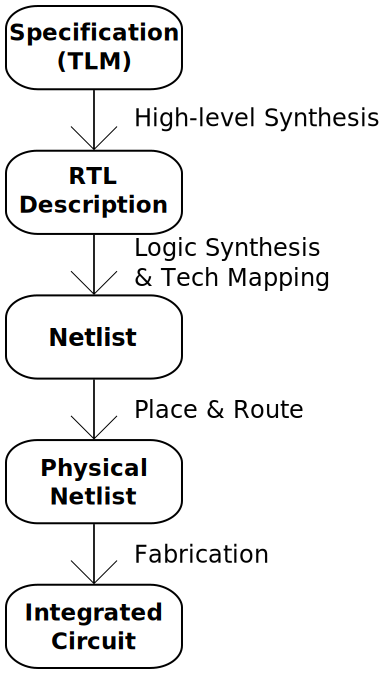
\includegraphics[width=0.5\textwidth]{./figures/designFlow}
}
\caption{Typical hardware design flow.}
\label{fig:cadflow}
\end{figure}
}

%\subsection{The Hardware Verification Imperative}
When moving from one abstraction level of the hardware design process to the 
next, an important issue arises: how can one ensure that the functionality of 
the optimized design matches original spec? 
Bugs in hardware design which are 
not caught early can have costly effects later, such as the need for a 
redesign. Bugs in arithmetic circuits can be especially catastrophic.
One infamous example is the 1994 floating point division (FDIV)
bug that affected the Intel Pentium chip \cite{nicely:FDIV}, 
and subsequently cost the company \$475 million because it was  
discovered after the chip's release. In another more fatal case, during the
Gulf war, an American Patriot Missile battery failed to intercept an incoming
enemy missile due to an arithmetic error \cite{arnold:patriot}.
Since hardware bugs can have significant consequences, 
there has been extensive work in field of hardware verification to find and
eliminate bugs prior to fabrication.

The two main methodologies used in hardware verification are simulation and 
formal verification. \emph{Simulation} checks correctness by applying exhaustive 
assignments to the circuit inputs and verifying correctness of the output. 
This ensures that the circuit performs as designed under all possible 
inputs. Such exhaustive testing is quite effective for smaller circuits. 
However, as the size of the circuit increases, it becomes 
computationally infeasible to simulate all possible test vectors. This is the 
case with Galois field arithmetic circuits, which are commonly very large in 
real-world applications. Often for such large circuits, simulations of a smaller and more 
manageable subset of test vectors are employed to catch bugs. While these tests
can increase confidence in the correctness of the design,  
{\it they do not guarantee correctness} since every data-flow of the design hasn't
been analyzed.
%Such is the case with large Galois field arithmetic circuits, so we instead 
%focus on formal verification. 

\section{Formal Verification}
Instead of simulating input vectors, \emph{formal verification} utilizes 
mathematical theory to reason about the correctness of hardware designs.
%which overcomes some limitations of simulation. 
Formal verification has two main forms: property checking and equivalence 
checking. 

{\it Property checking} (or property verification) verifies
that a design satisfies certain given properties. Property checking is done mainly 
in the form of theorem proving, model checking, or approaches which 
combine the two.
\begin{enumerate}
\item \emph{Theorem proving} \cite{theoremproving:91} requires the existence of
mathematical descriptors of the specification and implementation of the 
circuit. Theorem provers apply mathematical rules to these descriptors to
derive new properties of the specification. In this way, the tool can reduce
a proof goal to simpler sub-goals, which can be automatically verified.
However, generating the initial proof-goal requires extensive guidance from
the user, so there is an overall lack of automation in theorem 
proving.
\item \emph{Model checking} \cite{modelcheck:99} is an approach
to verifying finite-state systems where specification 
properties are modeled as a system of 
logic formulas. The design is then traversed to check if the 
properties hold. If the design is found to violate a
particular property, a counter-example is generated which exercises the
incorrect behavior in the design. Such counter-examples allow the designer
to trace the behavior and find where the error in the design lies.
Modern model checking techniques use the result to automatically refine
the system and perform further checking.
These tools are typically automated, and thus have found widespread 
use in CAD tool suites.
\end{enumerate}

{\it Equivalence Checking} verifies that two different representations of
a circuit design have equivalent functionality. An example of equivalence
checking as it applies to the hardware design flow is shown in
Fig. \ref{fig:equivflow}.

{
\begin{figure}[h]
\centerline{
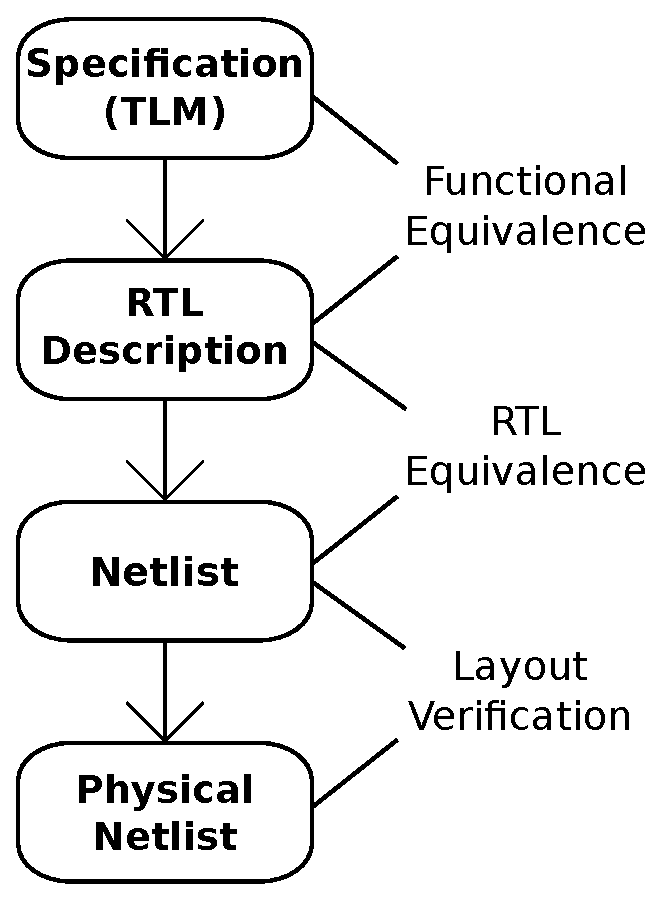
\includegraphics[width=0.5\textwidth]{./figures/designVerification}
}
\caption{Equivalence checking as applied to the hardware design flow.}
\label{fig:equivflow}
\end{figure}
}

There are two major
equivalence checking techniques: graph-based
and satisfiability-based.
\begin{enumerate}
\item \emph{Graph-based} techniques construct a canonical graph 
representation, such as a Binary Decision Diagram (\emph{BDD}) or one of
its many variants, of each circuit. A linear comparison is then conducted to 
determine whether the two graphs are isomorphic. Since the graph 
representation is canonical, the graphs of the two circuits will be 
equivalent if and only if the circuits perform the same function.
\item \emph{Satisfiability} techniques construct a miter of the two circuits,
typically in a graph such as an And-Inverter graph (\emph{AIG}). A
\emph{miter} is a combination of the two circuits with one bit-level output, which 
is only in a "1" state when the outputs of the circuits differ given 
the same given 
input, as shown in Fig. \ref{fig:miter}. 
A satisfiability (\emph{SAT}) tool \cite{csat} 
is then employed to simplify the graph and find a solution to the miter, 
i.e. find an input for which the 
miter output is "1". If a solution is found, this solution acts as a 
counter-example of when the circuit outputs differ; otherwise the circuits
are functionally equivalent.
\end{enumerate}


{
\begin{figure}[h]
\centerline{
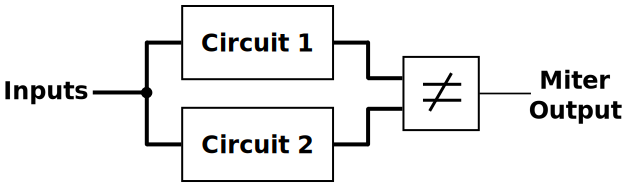
\includegraphics[width=0.8\textwidth]{./figures/betterMiter}
}
\caption{A miter of two circuits.}
\label{fig:miter}
\end{figure}
}

%\subsection{Computer-Algebra Based Formal Verification}
Certain formal verification methods use \emph{computer-algebra} and \emph{algebraic
geometry} techniques based on mathematical theories.
Unlike SAT-based verification, modern algebraic geometry 
techniques do not explicitly solve the constraints to find a solution; 
rather, they reason about the presence or absence of solutions, or explore
the geometry of the solutions.
These methods \cite{Avrunin:CAV} \cite{condrat-tacas07} \cite{gbverify:2007} 
transform the circuit design into a polynomial system. Typically, this system
of polynomials is then used to compute a Gr\"obner basis \cite{gb_book}. 
Computation of Gr\"obner bases allows for 
the easy deduction of important properties of a polynomial system, 
such as the presence or absence of 
solutions. These properties are then leveraged to perform 
verification. Unfortunately, such a computation 
has been shown to be doubly 
exponential in the worst case, and thus these methods have not been 
practical for real-world applications. However, recent
breakthroughs in computer-algebra hardware verification have shown
that it is possible to overcome the complexity of this computation while
still utilizing the beneficial properties of a Gr\"obner bases
\cite{lv:phd}.

\section{Importance of Word-level Abstraction}
Most formal verification techniques can benefit from word-level abstractions 
of the circuits they verify.
Abstraction is defined as state-space reduction, i.e{\text . }abstraction
reduces state-space by mapping the set of states of a system to a smaller 
set of states. Because the new representation contains fewer states, it
is easier to comprehend and thus easier to use. 
Word-level abstraction focuses specifically on abstracting a word-level
representation of a circuit out of a bit-level representation. For example,
a bit-level representation of an integer multiplier is represented by a
collection of Boolean inputs and outputs, whereas a word-level
abstraction hides the underlying logic and represents the circuit as two 
integer inputs and one integer output, e.g. $Z=A\cdot B$. As the bit-size of the
multiplier increases, the logical implementation of the multiplier grows (typically
exponentially) while the word-level abstraction stays the same.

Word-level abstractions have a wide variety applications in formal 
verification. Theorem proving techniques can leverage abstraction as an 
automatic decision procedure or as a canonical reduction 
engine. For example, since RTL is composed of circuit blocks that represent 
the underlying circuit, RTL verification methods can exploit 
abstractions of these blocks.
This is seen in the following RTL verification methods:
\begin{itemize}  
\item Model checking \cite{kroening:model}, 
where an approximation abstraction of RTL blocks is generated and then 
refined.
\item Graph-based equivalence 
checking \cite{WLS} \cite{arditi:bmd}, where abstraction methods are used
to generate a canonical word-level graph representation of the circuit.
\item Satisfiability-based equivalence checking \cite{lpsat}, where 
abstractions are used identify symmetrics and similarities in order to 
minimize the amount of logic that is sent to the 
SAT tool. 
\end{itemize}

Other equivalence checking techniques that employ abstractions 
include satisfiability modulo theory ({\it SMT}) techniques \cite{boolector} \cite{bryant:tacas07}, 
which are similar to SAT except they operate on higher-level data
structures (integers, reals, bit vectors, etc.), as well as 
constraint solving techniques \cite {ms:research} \cite{tew:iccad08}.
In general, RTL equivalence checking approaches would ideally maintain a 
high-level of abstraction while still retaining sufficient lower-level 
functional details  (such as bit-vector size, precision, etc) 
\cite{gupta_survey}.

Word-level hardware abstractions also have applications in RTL and datapath 
synthesis \cite{demicheli:iccad_98} \cite{demicheli:dac_99}
\cite{demicheli:tcad_03}. 
Abstractions of circuits allow for design reuse, which allows for tool-automated 
synthesis of larger circuit blocks.
Since hardware design specifications tend to be word-level, synthesis tools 
can use these larger circuit blocks to generate and optimize the
datapaths and create the RTL of the system. Thus, in order for a circuit to 
be used by these automated synthesis tools, its word-level abstraction must
be known.

Finally, abstractions can also be applied to detect malicious 
modifications to a circuit, potentially inserted as a hardware trojan horse.
Hardware trojans, a relatively new security concern in the hardware 
industry, use certain techniques to add incorrect behavior to a 
design. 
This behavior is only activated under certain rare circumstances that only 
the mal-intent designer has knowledge of.
The behavior is purposely hidden and is very difficult to encounter during 
simulation of the design. A manufactured chip with a subsystem 
that contains a hardware trojan could compromise the entire system in which 
it is used.
In some hardware trojan cases, formal verification techniques may be applied 
to catch a bug in a design and provide a counter-example which exercises it. 
However, it can be difficult to tell whether the bug in the design was 
introduced intentionally of not. On the other hand, word-level abstractions 
of bit-level circuits {\it effectively reverse-engineer the true function 
implemented by the circuit}, which could be used to determine the designer's 
true intention.

\section{Dissertation Objective, Motivation, and Contributions}
This dissertation focuses on abstracting a canonical, 
word-level representation of hardware (bit-level) implementations of 
combinational circuits. The proposed technique is a full abstraction solution which can be 
applied to any arbitrary acyclic combinational circuit. 
It is particularly efficient when applied to Galois field arithmetic circuits.
Using this technique, if the abstraction of the circuit's implementation and its
specification are found, they can be easily compared to determine equivalence.
Implementation of a custom software tool, developed to compute the abstractions, is
also described.

\subsection{Motivating Application}
The motivation for this work comes from applications of Galois field 
arithmetic circuits in elliptical curve cryptography ({\it ECC}) hardware systems.
The main operations of encryption, decryption, and 
authentication in ECC rely on operations performed on elliptic curves, which 
are implemented in hardware as polynomial functions over Galois fields. 
To be applicable in real-world situations, ECC data-paths
should be a minimum of $163$-bits wide, which is the minimum NIST standard, 
up to a recommended size of $571$-bit operand widths. Many non-ECC cryptosystems
have datapaths on the order of $1000$-bits.

A Galois field arithmetic circuit with a datapath size of $k$ 
is built as a Boolean function: $\mathbb{B}^k \rightarrow \mathbb{B}^k$. 
This function is mapped to an operation 
$f:\mathbb{F}_{2^k} \rightarrow \mathbb{F}_{2^k}$ 
over the Galois field $\mathbb{F}_{2^k}$. 
These circuits are custom-built, modular
systems which cannot be synthesized due to their complex nature. Thus, 
formal verification is needed to ensure they operate correctly.

Recent computer-algebra based formal verification techniques have been
able to perform verification of Galois field arithmetic circuits with
a datapath size up to $163$-bits \cite{lv:phd}. Word-level abstractions 
of Galois
field arithmetic circuits could be used to further improve these formal 
verification techniques to allow for verification of larger circuits, as
well as provide the other benefits of word-level abstraction.
However, there is currently no technique for computing word-level 
abstractions of Galois field circuits of any practical size.

{
\begin{figure}[h]
\centerline{
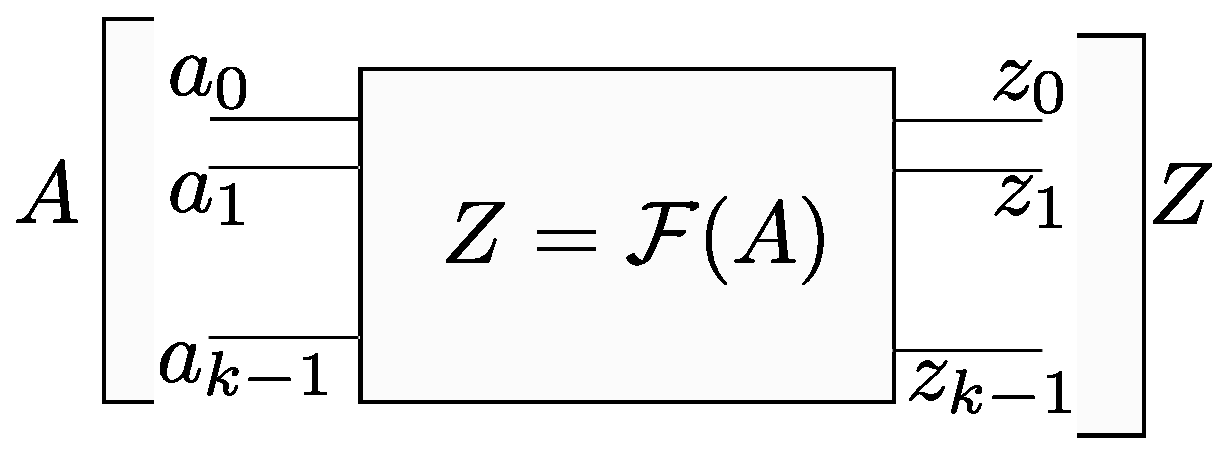
\includegraphics[width=0.5\textwidth]{./figures/interpolate}
}
\caption{Circuit with $k$-bit input $A$ and $k$-bit output $Z$. 
Abstraction to be derived as $Z=\Func(A)$.}
\label{fig:abstractA_Z}
\end{figure}
}

While the motivation comes from the need to verify Galois field arithmetic
circuits, the presented approach can be generalized to be applicable to any
combinational acyclic circuit.
Any such circuit with a $k$-bit input $A$ and a $k$-bit output $Z$, such
as the one shown in Fig. \ref{fig:abstractA_Z}, computes 
$f: \mathbb{B}^k \rightarrow \mathbb{B}^k$ and can thus be analyzed as the
function $f: \Fkk \rightarrow \Fkk$. Over $\Fkk$ this function can be 
represented as the polynomial $Z=\Func(A)$. This is trivially generalized
when there are multiple $k$-bit inputs $A_1,A_2,\dots,A_i$, i.e. $Z=\Func(A_1,\dots,A_i)$.
Now assume the word-size of the input differs from the output, that is the circuit
computes $f: \mathbb{B}^m \rightarrow \mathbb{B}^n$ for $m \neq n$. This can 
be represented as a function over Galois fields as $f: \F_{2^m} \rightarrow \F_{2^n}$.
This function can be analyzed over the field $\Fkk$ such that $\Fkk \supset \F_{2^m}$ 
and $\Fkk \supset \F_{2^m}$, where $k=LCM(m,n)$.

\subsection{Dissertation Contributions}
To solve the problem of word-level abstraction, this dissertation proposes 
a full solution consisting of three main contributions.

\begin{enumerate}
\item A theory for finding the word-level abstraction from a bit-level circuit over Galois fields is created.
The given bit-level circuit implementation is modelled as a system of
polynomials over the field.
This theory is derived using techniques from computer-algebra, notably the theory of
\Grobner basis \cite{pruss:iwls13}.
\item Using this theory, new algorithms based on symbolic computation are developed to 
derive the word-level abstraction. The algorithms are designed to be applicable to 
industry-size arithmetic circuits over Galois fields \cite{pruss:dac14}\cite{sun:date15}.
A complexity analysis of the algorithmic approach is also presented. Furthermore, the
approach is also generalized to make it applicable to arbitrary combinational circuits.
Finally, we show how the approach can be used to exploit the hierarchical structure of
large Galois field multipliers designed over composite fields.
\item A custom software tool implementation of the algorithmic approach is described, including
an analysis of efficient data structures designed for this purpose \cite{pruss:tcad15}.
\end{enumerate}

Experiments show that the proposed solution can abstract canonical, word-level, 
polynomial representations of Galois field arithmetic circuits up to $1024$-bits in
size, while other contemporary approaches are infeasible beyond a $32$-bit designs.


%an 
%approach based on computer-algebra, algebraic geometry - notably the theory of
%{\it Gr\"obner bases} \cite{gb_book} \cite{buchberger_thesis}.
%and {\it elimination ideals} \cite{ideals:book}, as our approach for 
%abstracting canonical word-level representations from bit-level Galois 
%field arithmetic circuits. 
%Computer-algebra techniques easily integrate with 
%Galois field theory and allow for polynomial abstraction of the circuit over 
%the field itself. Thus, if the circuit computes a function over some field $
%\mathbb{F}_{2^k}$, the resulting abstraction is a word-level polynomial 
%function over the same field $\mathbb{F}_{2^k}$. 

%The given bit-level circuit implementation is first modeled as a system of
%polynomials over the field. Using the theory of elimination ideals, we 
%derive an elimination term ordering and prove that by using this ordering we 
%can obtain a canonical word-level representation of a circuit by 
%computing a Gr\"obner basis of the polynomials. However, complexity 
%of the computation of a Gr\"obner basis proves to be prohibitive for circuits
%of practical size. Therefore, we employ a select sub-set of computations 
%from the Gr\"obner basis theory to overcome this complexity and obtain the
%abstraction. We prove that this simpler computation can be 
%performed via a polynomial reduction process, and engineer a custom 
%verification tool for this purpose. Using this approach, we are able to 
%successfully 
%abstract word-level representations of Galois field arithmetic circuits up 
%to $571$-bits, which is the {\it largest recommended NIST standard} for ECC.


\section{Dissertation Organization}
The rest of this dissertation is organized as follows. Chapter
\ref{ch:prev} reviews previous applicable work and highlights their
drawbacks with respect to the canonical, word-level abstraction problem. 
Chapter \ref{ch:prelim} describes the properties of Galois fields, 
$\mathbb{F}_{2^k}$, and explains the process of constructing them.
It also describes how to design arithmetic circuits over such fields, their 
complexities, and the role of these circuits in Elliptic Curve Cryptography.
Chapter \ref{ch:ideals} provides a theoretical background of 
computer-algebra and Gr\"obner bases and explains their application
to Galois fields. 
Chapter \ref{ch:abstract} describes an approach to abstract 
word-level polynomial representations of combinational circuits using a 
Gr\"obner basis computation.
Chapter \ref{ch:improv} improves on this word-level abstraction approach to 
make it applicable to much larger circuits.
Chapter \ref{ch:generalize} generalizes the abstraction approach to make
it applicable to circuits with varying operand word-lengths. It also describes how the 
approach can take advantage of the hierarchy of arithmetic circuits designed over
composite fields.
Chapter \ref{ch:implement} describes the implementation details of a 
custom abstraction tool and gives experimental results of
abstracting large Galois field multiplier circuits.
Chapter \ref{ch:concl} concludes the dissertation and outlines potential future 
research for continuation of this work. 

%\input{myformulae.tex}


\section{Preliminaries}

\subsection{FSM model for sequential circuits}
A finite state machine (FSM) is a mathematical model of computation for designing and analyzing sequential logic 
circuits. If a FSM's primary outputs depend on primary inputs and present state inputs, it is named as a \textit{Mealy machine};
the formal definition is as follows:
\begin{Definition}
A Mealy machine is an $n$-tuple $\mathcal M = (\Sigma,O,S,S^0,\Delta,\Lambda)$ where
\begin{itemize}
\item $\Sigma$ is the input label, $O$ is the output label;
\item $S$ is the set of states, $S^0\subseteq S$ is the set of initial states;
\item $\Delta:\ S\times\Sigma\to S$ is the next state transition function;
\item $\Lambda:\ S\times\Sigma\to O$ is the output function.
\end{itemize}
\end{Definition}
The other kind of FSM is \textit{Moore machine}, its difference from Mealy machine is that
its primary outputs only depend on the present states, i.e. the output function is defined as
$$\Lambda:\ S \to O$$
Typical sequential circuits can be depicted as Fig.\ref{fig:seqmodel}(a). Primary inputs
$x_1,\dots,x_m \in \Sigma$, and primary outputs $z_1,\dots,z_n\in O$. Signals $s_1,\dots,s_k$ 
are present state (PS) variables, $t_1,\dots,t_k$ are next state (NS) variables.
We can define 2 $k$-bit words denoting the PS/NS variables as there are $k$ flip-flops
in the datapath: $S = (s_1,\dots,s_k), ~T=(t_1,\dots,t_k)$. Transition function
at bit level are defined as $\Delta_i: t_i = \Delta_i(s_1,\dots,s_k,x_1,\dots,x_m)$.
\begin{figure}[hbt]
\centering{
%\begin{minipage}{12cm}
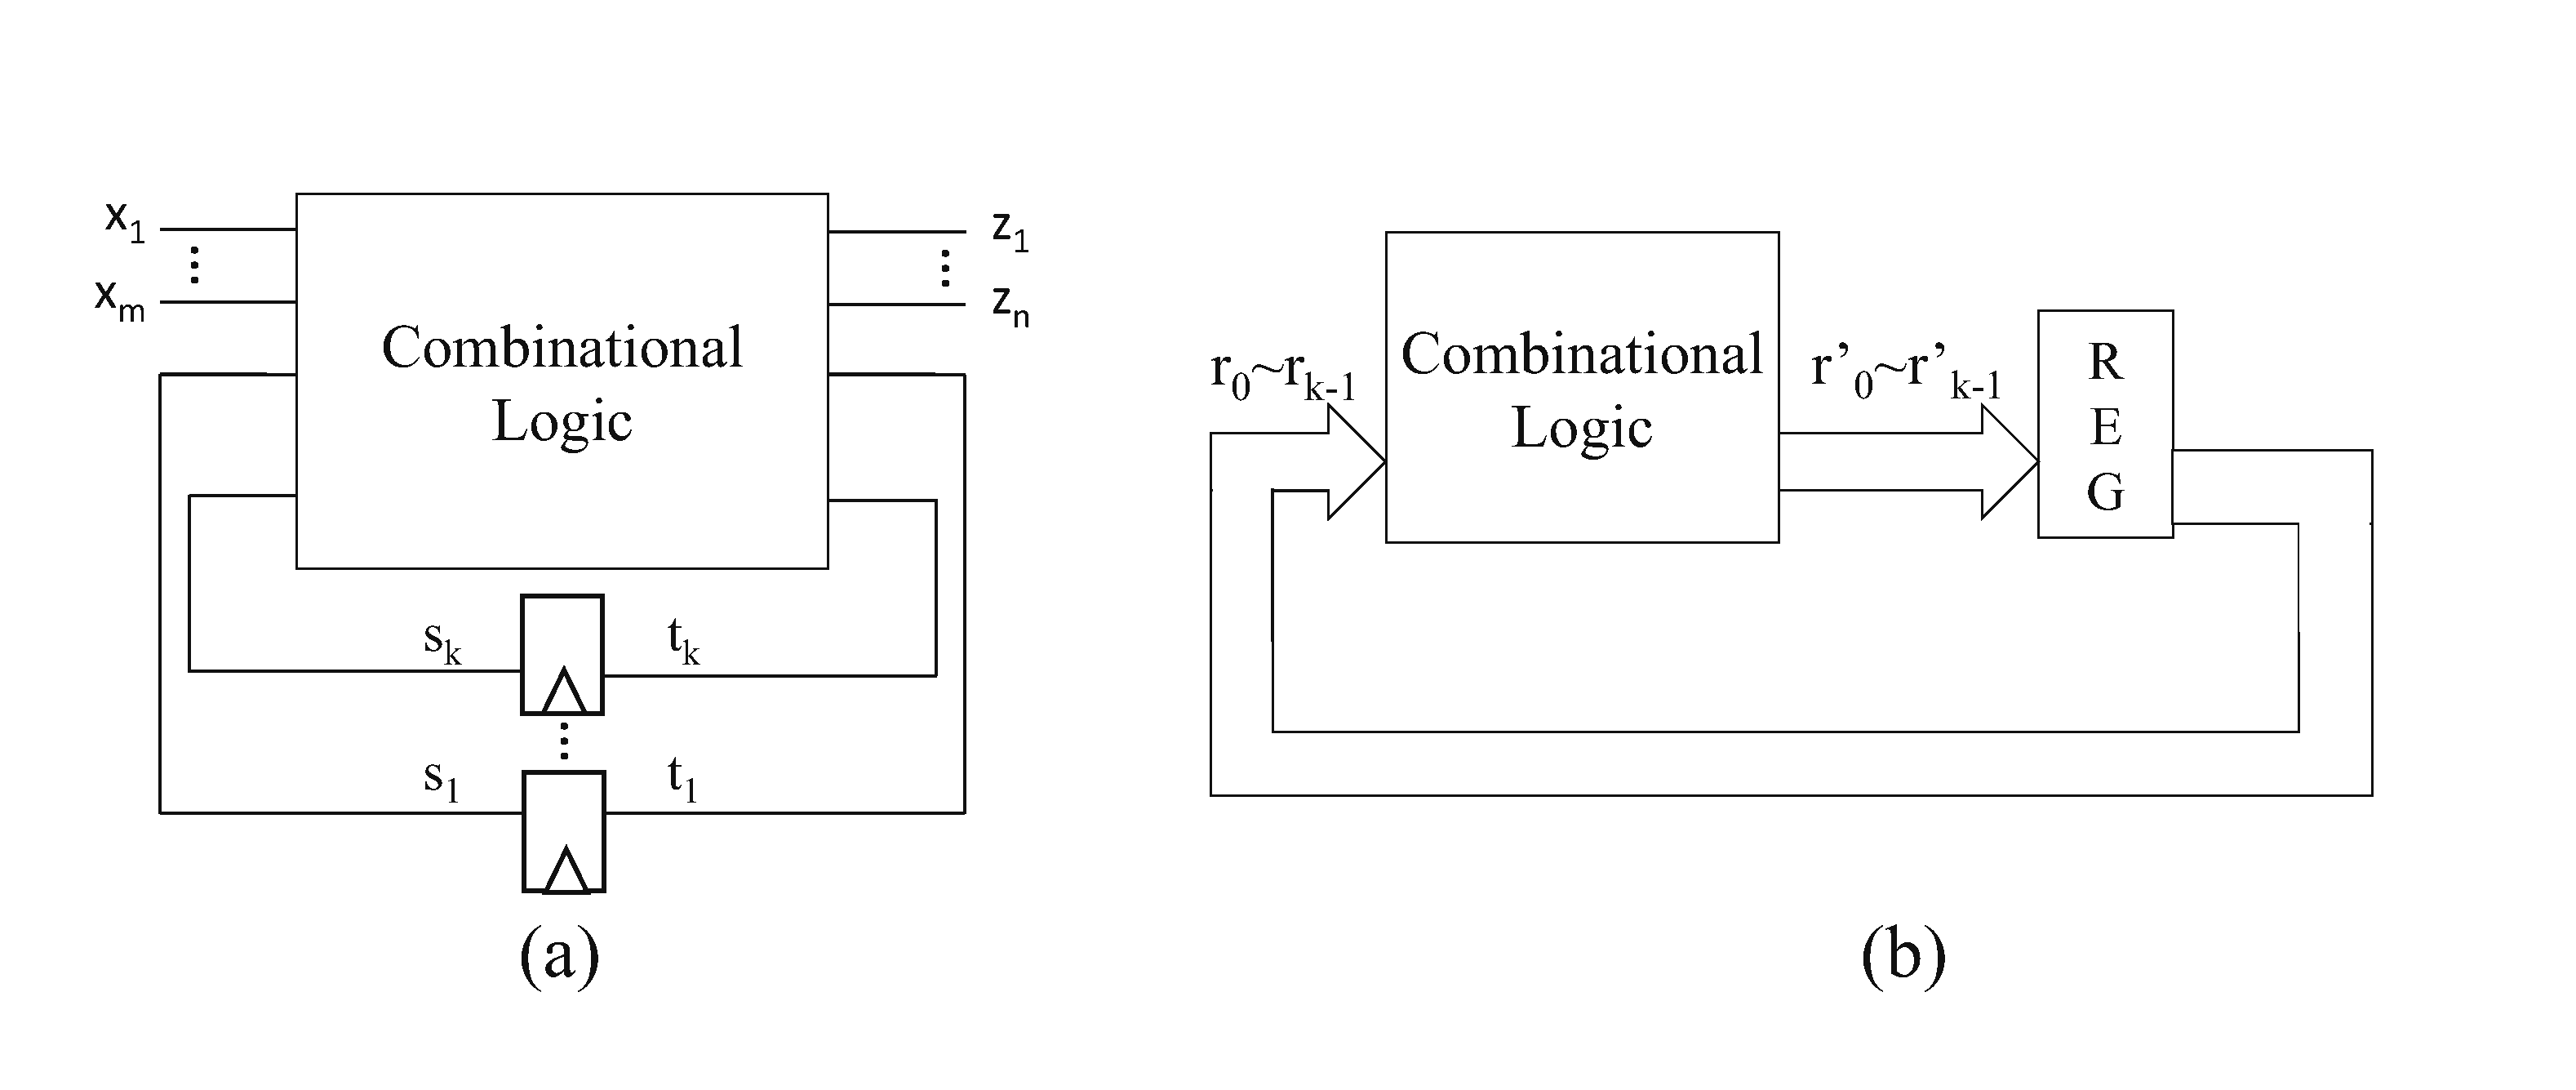
\includegraphics[width=3.5in]{./seqmodel.eps}
% \vspace{-0.2in}
\caption{FSM models of sequential circuits}
%\end{minipage}
\label{fig:seqmodel}}
\end{figure}
In some cases, arithmetic computations are implemented as Moore machines where input operands
are loaded into register files $R$ and the FSM is executed for $k$ clock cycles.
We can simplify them to the model in Fig.\ref{fig:seqmodel}(b).

\subsection{Commutative algebra and algebraic geometry preliminaries}
A {\bf field} $\mathbb{F}$ is a set of elements, including 0 and 1 (unity),
allowing for associative and commutative addition and multiplication;
and every non-zero element has a multiplicative inverse.  A {\bf
  finite field} or {\bf Galois filed} is a field with a finite number
($q$) of elements, and is denoted by $\Fq$, where $q=p^k$ is a power of
a prime integer $p$. In our work, $q = 2^k$ for
a given $k$, where $k$ represents the datapath (bit-vector)
word-lengths, or the number of memory elements (state registers) in
finite state machines. 

Let the field $\mathbb{F}_2 = \{0, 1\} ~(\equiv \B)$, and let
$\mathbb{F}_2[X]$ denote the set (ring) of all univariate polynomials
in variable $X$ with coefficients from $\mathbb{F}_2$. Then, the
Galois field $\Fkk$ is constructed as $\Fkk = \mathbb{F}_2[X] \pmod{
  P(X)}$, where $P(X)$ is an irreducible polynomial over
$\mathbb{F}_2$. Let $\alpha$ be a root of the irreducible polynomial
$P(X)$, i.e. $P(\alpha) = 0$. Any element $A \in \Fkk$ can be
represented as $A = \sum_{i=0}^{k-1} a_i \alpha^i$, where $a_i \in
\mathbb{F}_2$. The field $\Fkk$ is therefore, a $k$-dimensional {\it
  extension} of the base field $\mathbb{F}_2$: so,  $\mathbf{\Fkk \supset
\mathbb{F}_2}$. Consequently, all operations of addition and
multiplication in $\Fkk$ are performed modulo the irreducible
polynomial $P(\alpha)$ and coefficients are reduced modulo 2.  

Boolean variables in field $\mathbb B$ can be easily mapped to
elements in $\mathbb F_2$. Since $\mathbb F_2 \subset \Fkk$, these 
%Namely $k$-bit Boolean bit-vector defined
%over Boolean ring $\mathbb B^k$ can also be mapped uniquely  to $\Fkk
%= \mathbb F_2[x_1,\dots,x_k]$. 
Boolean operators are interpreted as functions over $\Fkk$ (where $+$
and $\cdot$ are addition and multiplication performed modulo 2): 
\begin{align*}
&a\land b \to a\cdot b\\
&a\oplus b \to a+b\\
&\neg a \to 1+a\\
&a \bar{\oplus} b \to 1+a+b\\
&a \lor b \to a+b+a\cdot b
\end{align*}

Using these mappings we can write Boolean functions in form of
polynomials over $\mathbb F_2\subset \Fkk$. 
These concepts provide a mechanism to represent and
manipulate both bit-level ($\mathbb{F}_2$) and $k$-bit word-level
constraints {\bf in one unified mathematical domain $\Fkk$ --- a
  concept we   exploit for abstraction. }
  Consider Ex.\ref{ex:motiv},
polynomials for transition functions (bit-level outputs) $f_1,f_2$
are over $\mathbb F_2$, i.e. $f_1,f_2\subseteq \mathbb F_2 \subset \Fkk$,
and polynomials containing word-level variables $f_3,f_4,f_5 \subseteq \Fkk$.
All polynomials belong to unified domain $f_1,f_2,\dots,f_5 \subseteq \Fkk$.

It is well-known that every Boolean mapping between $k$ dimensional
Boolean spaces $f: \B^k \rightarrow \B^k$ can be construed as a
function over Galois fields $f: \Fkk \rightarrow \Fkk$. Moreover,
every function $f: \Fkk \rightarrow \Fkk$ is a polynomial function: 
i.e. $f$ can be represented by way of a unique, minimal, canonical
polynomial $\F(X)$, and the work of \cite{timDAC} shows how to
efficiently derive such polynomial representations from circuits ---
another concept that makes our approach feasible. 


We represent Boolean circuits by way of polynomials over
$\Fkk$. If we take indeterminates $x_1,x_2,\dots,x_n$, an arbitrary
combination of their finite product  
$x_1^{d_1}\cdot x_2^{d_2}\cdots x_n^{d_n}, d_i\geq 0$ 
is a {\bf monomial}. A {\bf polynomial} $f = c_1 X_1 + c_2 X_2 + \dots
+ c_t X_t$ is a finite sum of terms, where $c_1, \dots, c_t$ are
coefficients and $X_1, \dots, X_t$ are monomials. The set of {\it all}
such polynomials with coefficients from $\Fkk$ forms a {\bf
  multivariate polynomial ring} denoted $\Fkk[x_1,\dots,x_n]$. 
A monomial ordering $X_1 > X_2 \dots > X_t$ is imposed on the
polynomials to process them systematically. Then, $LT(f) = c_1 X_1,
LM(f) = X_1$ denote the leading term and the leading monomial of $f$,
respectively. 


Multivariate polynomial division will play a key role in our
algorithmic techniques. Division is implemented as {\it cancellation
  of terms.} Given polynomials $f, g$, if $cX$ is a term in
$f$ that is divisible by $LT(g)$, then $f \xrightarrow{g} r$ denotes a
one-step reduction (division) of $f$ by $g$, resulting in remainder $r
= f - {{cX} \over {LT(g)}} \cdot g$. This has the effect of cancelling
the term $cX$ from $f$. 
\begin{Example}
\label{ex:multidiv}
If $f = e + cd$ and $g = c + ab$,
then the term $cd$ in $f$ can be canceled by $LT(g) = c$: $r = f - {cd
  \over c} g = e + abd$. 
\end{Example}
  Similarly, $f$ reduces to $r$ modulo the set
of polynomials $F = \{f_1, \dots, f_s\}$, denoted $f \stackrel{F}
{\textstyle   \longrightarrow}_+ r$, such that no term in $r$ is
divisible (cancellable) by the $LT(f_i)$ of any polynomial in $ f_i
\in F$.    


In verification, we have to analyze the {\it solutions to a
set of polynomials.} The set of all solutions to a system of
polynomial equations $f_1 = \dots = f_s = 0$ is defined as the affine variety:
\begin{Definition}
Given a set of polynomials $f_1,\dots,f_s$ over ring $\mathbb F_q[x_1,\dots,x_n]$, their 
{\bf affine variety} 
$$V(f_1,\dots,f_s) = \{(a_1,\dots,a_n)\in  (\mathbb F_q)^n |
f_1(a_1,\dots,a_n) = \cdots = f_s(a_1,\dots,a_n) = 0\}$$ 
\end{Definition}

Generally we can find many sets of polynomials with the same variety, which are linear combinations
of given set of polynomials. This set is defined as follows:
\begin{Definition}
{\bf Ideal of Polynomials:} Let $f_1,f_2,\dots,f_s\in \mathbb F[x_1,\dots,x_n]$.
Define an ideal
$$J = \langle f_1,f_2,\dots,f_s\rangle = \{f_1\cdot h_1 + f_2\cdot h_2 +\cdots + f_s\cdot h_s : h_1,\dots,h_s\in \mathbb F[x_1,\dots,x_n]\}$$
We call $J = \langle f_1,f_2,\dots,f_s\rangle$ an ideal generated by $f_1,\dots,f_s$ and these polynomials 
the {\bf generators} of ideal $J$.
\end{Definition}
% On the other hand, if given another polynomial $f$, we need to judge whether it belongs to $J$.
A practical problem is: given an ideal $J = \langle f_1,f_2,\dots,f_s\rangle$ and a polynomial $f$,
we need to check if the variety of $J$ can make the evaluation of $f$ equal to 0, i.e. $f$ vanishes on $V(J)$.
This problem is usually described as ideal membership checking problem.
\begin{Definition}
{\bf Ideal membership:} Let $f_1,f_2,\dots,f_s\in \mathbb F[x_1,\dots,x_n]$, and $J = \langle f_1,f_2,\dots,f_s\rangle$
be an ideal over ring $\mathbb F[x_1,\dots,x_n]$. If 
$$f = f_1h_1 + f_2h_2 + \cdots + f_sh_s$$
then $f\in J$.
\end{Definition}

An ideal may have many generating sets. For example, we may have different set of polynomial generators denoting
the same ideal, where they have the same variety: $\langle f_1,\dots,f_s\rangle = \langle h_1,\dots,h_r\rangle
= \langle g_1,\dots,g_t\rangle$ such that $V(f_1,\dots,f_s) = V(h_1,\dots,h_r) = V(g_1,\dots,g_t)$.
Therefore a canonical representation of an ideal is needed, which leads to the concept of Gr\"obner bases.

\begin{Definition}
The set $G = \{g_1, \dots,
g_t\}$ is called a \textbf{\Grobner basis} of $J$ if and only if the
leading term of all polynomials in $J$ is divisible be the leading
term of some polynomial $g_i$ in $G$: i.e. $\forall f \in J, \exists
g_i \in G \ s.t. \ LT(g_i) ~|~ LT(f)$. 
\end{Definition}
% The famous Buchberger's
% algorithm, given in textbook \cite{ideals:book}, is used to compute a
% \Grobner basis (GB). Operating on  input $F = \{f_1, \dots, f_s\}$,
% and subject to the imposed term order $>$, it derives $G = GB(J) = \{
% g_1, \dots, g_t \}$. Buchberger's algorithm repeatedly computes
% $S$-polynomials. For pairs $(f_i, f_j) \in F$, $Spoly(f_i, f_j) =
% \frac{L}{lt(f_i)}\cdot f_i - \frac{L}{lt(f_j)}\cdot f_j$, where $L =
% LCM(LM(f_i), LM(f_j))$. Reducing $Spoly(f_i, f_j) \xrightarrow{F}_+ r$
% cancels the leading terms of $f_i, f_j$ and gives a polynomial $r$
% with a new leading term. This remainder $r$ is added to the current
% basis and $Spoly(f_i, f_j)$ computations are repeated for all pairs of
% polynomials until all $S$-polynomials reduce to 0.  

An advantage of representing an ideal with GB is that it can serve as a decision procedure for ideal membership
test when dividing a polynomial $f$ by a GB, i.e.
$$G = GB(J) \Longleftrightarrow \forall f\in J, f\xrightarrow{g_1,g_2,\dots,g_t}_{+} 0$$
Gr\"obner basis can be reduced by eliminating redundant elements. \textbf{A reduced GB is a canonical representation of 
the ideal under a given monomial ordering}. Given an ideal $J = \langle f_1,\dots,f_s\rangle, ~G = 
\{g_1,\dots,g_t\}$ is the GB of $J$, it can be computed by Buchberger's algorithm (refer to textbook \cite{ideal:book}).

Another advantage of using GB representation is that GB computation can work as a {\it quantification procedure}.
In the following part we will introduce the concept of \textit{vanishing polynomials}, \textit{elimination ideal}, etc.
as the bases of this theory.

{\it Fermat's little theorem over $\Fq$:} For any $ \alpha \in \mathbb
F_{q}, \alpha^q = \alpha$. Therefore, the polynomial $x^q - x$
vanishes ($=0$) over $\Fq$, and is called a vanishing polynomial. We
denote by $J_0 = \langle x_1^q - x_1, \dots, x_d^q - x_d \rangle$ the
ideal of all vanishing polynomials in $\Fq[x_1, \dots, x_d]$. When $q
= 2^k, x^q - x = x^q + x$ as $-1 = +1$ over $\Fkk$.

Gr\"obner bases can be used to {\it eliminate} (i.e. quantify) variables from an
ideal. Given ideal $J = \langle f_1,\dots,f_s\rangle \subset \mathbb
F_{q}[x_1,\dots,x_d]$, the $l^{th}$ elimination ideal $J_l$ is the
ideal of $\Fq[x_{l+1}, \dots, x_d]$ defined by $J_l = J \cap
\Fq[x_{l+1}, \dots, x_d]$. Variable elimination can be achieved 
by computing a Gr\"obner basis of $J$ w.r.t. elimination orders: 
\begin{Theorem}
\label{thm:elim}
(Elimination theorem\cite{ideals:book}) Let $J\subset \mathbb
  F_{2^k}[x_1,\dots,x_d]$ be an ideal and let $G$ be a Gr\"obner basis
  of $J$ with respect to a lexicographic (LEX) ordering where
  $x_1>x_2>\cdots>x_d$. Then for every $0\leq l\leq d$, the set $G_l =
  G\cap\mathbb F_{2^k}[x_{l+1},\dots,x_d]$ is a Gr\"obner basis of
  the $l$-th elimination ideal $J_l$.
\end{Theorem}
We describe an application of elimination ideals using following example borrowed from \cite{ideals:book}:
\begin{Example}
Consider polynomials $f_1: x^2-y-z-1;\ f_2:x-y^2-z-1;\ f_3:x-y-z^2-1$ and ideal $J = \langle f_1,f_2,f_3\rangle
\subset \mathbb C[x,y,z]$. Gr\"obner basis $G = GB(J)$ w.r.t. LEX term order equals to 
$g_1:x-y-z^2-1;\ g_2:y^2-y-z^2-z;\ g_3: 2yz^2-z^4-z^2;\ g_4:z^6-4z^4-4z^3-z^2$. From observation,
we find that the polynomial $g_4$ only contains variable $z$ ($x,y$ eliminated), and polynomials $g_2,g_3,g_4$ only contain variables
$y,z$ ($x$ eliminated). According to theorem \ref{thm:elim}, $G_1 = G\cap\mathbb C[y,z] = \{g_2,g_3,g_4\}$
is the Gr\"obner basis of the $1^{st}$ elimination ideal of $J$ and $G_2 = G\cap\mathbb C[z] = \{g_4\}$ is the 
$2^{nd}$ elimination ideal of $J$, respectively.
\end{Example}

\subsection{Application of elimination theorem on circuit verification}
\label{sec:elim}
Assume that we are given a circuit (combinational component) with input $A = (a_0,\dots,a_{k-1})$ and output 
$R = (r_0,\dots,r_{k-1})$ (both can be represented
by word level variables in $\Fkk$). We can describe this circuit with an elimination ideal $J+J_0$, where
$J$ is the ideal generated by the polynomials corresponding to circuit gates and $J_0$ is the ideal of vanishing polynomials.
The authors of \cite{timDAC} showed that for any combinational
logic block, a canonical word-level polynomial representation can be
derived through \Grobner bases computed with elimination orders:
\begin{Lemma}
(From \cite{timDAC}) Given a combinational circuit $C$ with $k$-bit
  input $A = (a_0, \dots, a_{k-1})$ and $k$-bit output $R = (r_0, \dots,
  r_{k-1})$. Denote by $x_1, \dots, x_d$ all the bit-level
  variables of   $C$. Let $J = \langle f_1, \dots, f_s \rangle \subset
  \Fkk[x_1, \dots, x_d, R, A]$ denote all the polynomials corresponding to the
  logic gates of the circuit. Let $J_0 = \langle x_1^2 - x_1, \dots,
  x_d^2 - x_d, R^q - R, A^q - A \rangle$ be the vanishing ideal, so
  that $J + J_0 = \langle f_1, \dots, f_s, ~~ x_1^2 - x_1, \dots,
  x_d^2 - x_d, R^q - R, A^q - A \rangle$. Compute \Grobner basis $G =
  GB(J + J_0)$ w.r.t. lex term order with $x_1 > x_2 > \dots > x_d > R
  > A$. Then $G_d = G \cap \Fkk[R, A]$ eliminates the internal
  variables $x_1, \dots, x_d$ of the circuit. $G_d$ also contains the
  word-level polynomial $R = \F(A)$ which canonically represents the
  function of the circuit with only word level variables $R$ and $A$.
\end{Lemma}
This lemma shows an application of GB computations over an elimination ideal.
Since it abstracts the function of a combinational circuit, we call the term order
$primary~inputs~and~intermediate~variables~>~word~level~output~>~word~level~inputs$
as \textit{abstraction term order} (ATO).
If we further eliminate word-level input, the result will be a polynomial containing only 
the word-level output variable. In a sequential circuit
such as Ex.\ref{ex:motiv}, the output of combinational logic serves as the next state variable. Polynomial $g_T$ in
the example is the desired projection; i.e. using GB computation on elimination ideal and eliminating to NS
variables provides us the canonical representation of reachable states in next time frame.



% Machine traversal is key for many verification techniques, e.g. to check
% the equivalence of 2 FSMs, we can observe whether the output responses are the same at
% every step of traversal. An explicit traversal is usually infeasible, here we use 
% implicit state enumeration (BFS traversal) based on Boolean formulas to implement a machine traversal.
% The algorithm is as follows:
% \begin{algorithm}[hbt]
% \SetAlgoNoLine
%  \KwIn{Transition functions $\Delta$, initial state $S^0$}
% 
%   $from^0 = reached = S^0$\;
%   \Repeat{$new^i == 0$}
%   {
%   	$i \gets i + 1$\;
% 	$to^i \gets$Img$(\Delta, from^{i-1})$\;
% 	$new^i \gets to^i \cap \overline{reached}$\;
%   	$reached \gets reached \cup new^i$\;
% 	$from^i \gets new^i$\;
%   }
% \Return{$reached$}
% \caption {Breadth-first Traversal Algorithm for Reachability Analysis of FSMs}\label{alg:BFS}
% \end{algorithm}
% The main computation in this algorithm is the \textit{image function}. Img$(\Delta,from^{i-1})$
% denotes the forward image of the set $from^{i-1}$ under the transition function $\Delta$.
% Let  $\Delta_i$ denote the transition relation 
% for $i^{th}$ bit of output $T$ (denoted by $t_i$), and it is described by a Boolean function. We can obtain the transition relation 
% for bit-vector $T$: $Tran(s_0,s_1,x,t_0,t_1) = \bigwedge_{i=1}^{2}(t_i\ \bar{\oplus}\ \Delta_i)$. Assume present states
% are represent by Boolean formulas $PS(s_0,s_1)$, then the image function is written as
% $\text{Img}(Tran,\ PS) = \exists_{s_0,s_1}\exists_{x}[Tran(s_0,s_1,x,t_0,t_1)\land PS(s_0,s_1)]$, where
% $\exists_x f$ denotes the existential quantification of $f$ w.r.t. $x$.
% \begin{Example}
% We use implicit state enumeration based on Boolean formulas to traverse FSM in Fig.\ref{fig:fsm}.
% Initial state $\{00\}$ can be represented by Boolean formula $C(s) = \overline{s_0}\cdot \overline{s_1}$.
% Transition function for $NS$ variables are 
% $$t_0\overline{\oplus}\Delta_0 = t_0\overline{\oplus}(\overline{x}\overline{s_0}\overline{s_1}+s_0s_1)$$
% $$t_1\overline{\oplus}\Delta_1 = t_1\overline{\oplus}(x\overline{s_0}+s_0\overline{s_1})$$
% \end{Example}
\section{On Unsatisfiable Cores of Ideals with Empty Variety}

Consider the polynomial ring $\Fkk[x_1, \dots, x_n]$, and an ideal $J$
generated by a set of polynomials $F = \{f_1, \dots, f_s\},
\idealj$. Suppose that it is known that $V(J) = \emptyset$, or
otherwise it is determined so by applying the Gr\"obner basis
algorithm. Throughout this document, we will assume that the set $F$
is such that $V(f_1, \dots, f_s) = \emptyset$, unless stated
otherwise. An interesting (and important) problem to solve is as
follows:   

\begin{Problem}
Identify a subset of polynomials $F_c \subseteq F, J_c = \langle F_c
\rangle$, such that $V(J_c) = \emptyset$ too. For lack of a better
term, let us call $F_c$ the infeasible core or the unsatisfiable
core (UNSAT core) of $F$. The terminology is borrowed from the domain of
Boolean Satisfiability solvers. If you can think of a better
terminology, please let me know. 
%Here $F_c = \{f_i : f_i \in F, i\leq s\}$.
\end{Problem}

UNSAT cores have important uses in post-verification debugging, and in
many abstraction-and-refinement techniques used in the analysis of
circuits and systems. Any contribution here will be important. 

\begin{Example}\label{ex1}
Consider the following set of polynomials:
\begin{align*}
f_1: & ab\\
f_2: & ab+a\\
f_3: & ab+b\\
f_4: & ab+a+b+1\\
f_5: & xy+y+x+1\\
f_6: & yz+y+z+1\\
f_7: & c + d\\
f_8: & c + d + 1
\end{align*}

Let $F = \{f_1, \dots, f_8\}$ and $J = \langle F \rangle \subseteq
\F_2[a, b, c, d, x, y]$ where $\F_2 = \{0, 1\}$. Then
$V_{\overline{\F_2}}(J) = \emptyset$ as $GB(J) = \{1\}$. 

Now consider the subset $F_c = \{f_1, \dots, f_4\}, J_c = \langle
F_c\rangle$; it turns out that $V_{\overline{\F_2}}(J)= \emptyset$ as
well, so $F_c$ is an UNSAT core of $F$. Likewise, $\{f_7, f_8\}$ also
form a core. 
\end{Example}


Any set of polynomials $F$ with empty variety is an UNSAT core in
itself. There may be more than one UNSAT cores in $F$, some
polynomials may or may not be common to multiple cores (i.e. these
cores may be non-disjoint), and these cores may have
different cardinalities (different $|F_c|$). The UNSAT core problems
are therefore further classified as: 
\bi
\item Identify a {\it minimum} core, i.e. a core of minimum
  cardinality. In Ex. \ref{ex1}, the set $\{f_7, f_8\}$ is a minimum
  core. [Hardest problem to solve?]
\item Identify a {\it minimal} core. An UNSAT core $F_{c}$ is minimal
  with respect to the property that while the variety of $F_{c}$ is
  empty, the variety of {\it any} subset of $F_c$ is {\it non-empty},
  i.e. $V( F_{c} - \{f_i\} ) \neq \emptyset$ for any $f_i \in
  F_c$. The set $\{f_1, \dots, f_4\}$ constitutes a minimal
  core. [Very important problem, but I guess still a Hard Problem to
    solve!] 
\item Identify any UNSAT core disregarding minimality; i.e. find any
  subset $F_c$ of $F$. For very large problems, sometimes it is
  beneficial to solve this problem, so long as we can experimentally
  demonstrate that the obtained cores are small and their size is close to
  minimal cores --- but maybe algorithmically they can be found very
  quickly/efficiently, whereas finding minimal/minimum cores may be
  computationally infeasible. 
\ei


\begin{Conjecture}
Buchberger's algorithm, and only 1 iteration of it, could be used to
identify a {\it minimal} core. 
\end{Conjecture}

\begin{Conjecture}
Buchberger's algorithm may also be used to identify a {\it minimum}
core, but it will probably require the enumeration of all cores. 
\end{Conjecture}

So,
let us ignore the {\bf minimum} core problem for now, and concentrate
on the {\bf minimal} one. 

The UNSAT core problem should be related to Gr\"obner bases. Suppose
that we are given $F_c = F - \{f_j\}$. Then, if $GB(F) = \{1\}$ and if
$GB(F_c) = \{1\}$ too, then doesn't it imply that $f_j \in \langle F_c
\rangle$? My reasoning is as follows: Denote $J = \langle F \rangle,
J_c = \langle F_c \rangle$. Since $V(J) = V(J_c) = \emptyset$, from
the Weak Nullstellensatz we have $J = J_c = \Fkk[x_1, \dots,
  x_n]$. This implies that $f_j$ can be composed of polynomials of
$F_c$, or $f_j \in F_c$. So $f_j$ is not part of the UNSAT core and
that can be identified using Gr\"obner bases. [Florian: Do you have a
  better/cleaner argument for this?]

\section{Investigating Algorithms to find UNSAT cores $F_c$ from $F$}

A n\"aive way (and inefficient way) to identify {\it a minimal core}
using the GB computation is given in Algorithm 1. In the algorithm, we
pick a polynomial $f_i$ and see if $V(F_c - \{f_i\}) = \emptyset$
(i.e. $F_c - \{f_i\}$ is also infeasible/UNSAT). If so, discard $f_i$
from the core; otherwise keep $f_i$ in the 
core. Pick a different $f_i$ and continue until all polynomials $f_i$
are visited. This algorithm {\it will produce a minimal core}, as we
have tested each polynomial $f_i$ for inclusion in the core. This
requires $O(|F|)$ calls to the GB engine, which is really impractical. 



\begin{algorithm}[hbt]
\caption{Find a minimal UNSAT core}\label{alg:MUS}
\label{alg1}
\begin{algorithmic}

 \REQUIRE{$F=\{f_1,\dots,f_s$\}, $J = \langle F \rangle$ } 
 \ENSURE{The minimal core $F_c \subset F$}
  %%%%%%%%%%%%%%%%%%%%
 \STATE{/* First of all, set $F$ as the core itself*/\;}
 \STATE{$F_c \gets F$;} 

 \FORALL{$f_i \in F_c$}
   \IF{ $\text{Gr\"obnerBasis}(F_c - \{f_i\}) = \{1\}$ } 
     \STATE{/* Discard polynomial $f_i$ as it does not belong to the core*/\;}
     \STATE{$F_c \leftarrow F_c - \{f_i\}$\;}
   \ELSE 
     \STATE{ Keep $f_i$ in the minimal core\;}
   \ENDIF
 \ENDFOR
 \RETURN {$F_c$ as the core}
\end{algorithmic}
\end{algorithm}


The question is if we can identify a core by analyzing the
$Spoly(f_i,f_j)\xrightarrow{F}_+1$ computation itself? Note here
that since $F$ is an UNSAT core, there definitely exists one iteration
of Buchberger's algorithm where $Spoly(f_i, f_j) \xrightarrow{F}_+ 1$
is achieved. We think that a core can definitely be found, and we will
show you how. Then we need to investigate further whether our approach
can be used to identify minimal cores without invoking the GB engine
multiple times. 

Recall that each step of division $f \xrightarrow{f_i}_+r$ operates as
$r = f - \frac{lt(f)}{lt(f_i)} f_i$. If $f$ is to be divided by (say)
two polynomials $f_i, f_j$, then: i) first we see if $lt(f_i) ~|~
lt(f)$. If so, then $lt(f)$ is canceled by $lt(f_i)$. ii) Otherwise,
we check to see if $lt(f_j)$ cancels $lt(f)$. This implies that while
performing the division $f \xrightarrow{f_1, \dots, f_s}_+r$, we can
identify (or keep track of) which polynomials in $f_1, \dots, f_s$ are
used to cancel terms of $f$. 

I will demonstrate the core identification with an Example.

\begin{Example}
Consider the set $F = \{f_1, \dots, f_8\}$ given in Ex
\ref{ex1}. Assume that our term order is LEX with $a > b > c > d > x >
y$.  Apply Buchberger's algorithm to $F$. 

\ben
\item Suppose that in the first
iteration $Spoly(f_1, f_4) \xrightarrow{F}_+r_1$ is computed. 
$Spoly(f_1, f_4) = a+b+1 = r_1$. Mark $f_1, f_2$ and keep them in the
set $F_m = \{f_1, f_4\}$. Since no polynomial
in $F$ divides $r_1$, we have $Spoly(f_1, f_4) \xrightarrow{F}_+ r_1 =
a+b+1$. No other polynomials (divisors) are marked. 

\item Update $F = F \cup r_1$

\item In the next iteration of Buchberger's algorithm, suppose we pair
  $r_1$ with $f_4$, and obtain  $Spoly(r_1, f_4)  = a + b^2 +
  1$. Polynomial $a+b^2+1$ is divisible by $r_1$, so $Spoly(r_1,
  f_4)\xrightarrow{F}_+r_2$, where $r_2 = b^2 + b$. Since $r_1$ is not
  a polynomial from the original set (it is derived from $f_1, f_4$),
  it is not marked. Update $F = F \cup r_2$, and the set of marked
  polynomials is still $F_m = \{f_1, f_4\}$.

\item Let us draw a graph representing this sequence of
  computations. This is shown in Fig. \ref{fig:trace} (a). The
  vertices (nodes) in the graph represent polynomials (marked or
  unmarked). Every vertex (polynomial) has either 0 or 2 incoming
  edges representing the $Spoly$ pair that derived it. It may also
  represent the remainder obtained from the dividend and the divisor
  (e.g. $a+b^2+1 \xrightarrow{a+b+1}_+ b^2+b$). [This graph is just to
    illustrate a book-keeping procedure].

\item We continue: Suppose that Buchberger's algorithm picks
  $S(f_1, f_2)  = a$. Now $r_1$ divides $a$, so $S(f_1, f_2)
  \xrightarrow{r_1}_+ r_3 = b+1$. $F = \{f_1, \dots, f_8, r_1, r_2,
  r_3\}$. Mark $f_1, f_2$ so that $F_m = \{f_1, f_4, f_2\}$. 
\item Next, $Spoly(f_1, f_3) = b$, and $b\xrightarrow{r_3}_+1$. Bingo!
  Mark $f_1, f_3$, $F_m = \{f1, \dots, f_4\}$.  Note that  $r_3$ is not marked as
  it is a derived polynomial. 

\item Update the graph, as  shown in Fig. \ref{fig:trace} (b).


\item Now, starting from the \textbf{1} node, traverse the graph
  backwards, to reach/identify all the vertices that are sources,
  i.e. those that have no incoming edges. Clearly, vertices 1, 2, 3, 4
  are the source vertices in this case. Of these vertices, identify
  only those that are marked in $F_m$. In this special case, all 4 of
  them are marked; so the core is obtained as $F_c = F_m$; in general, 
  we would only chose the marked vertices in the core. 

\item Just for fun, and to prove a point, compute $S(f_5, f_6)
  \xrightarrow{F}_+0$, so nothing is added to the Spoly graph. On the
  other hand, $Spoly(f_7, f_8)$ would have given us the   minimum
  core. 
\een

\end{Example}



\begin{figure}[hbt]
\centering
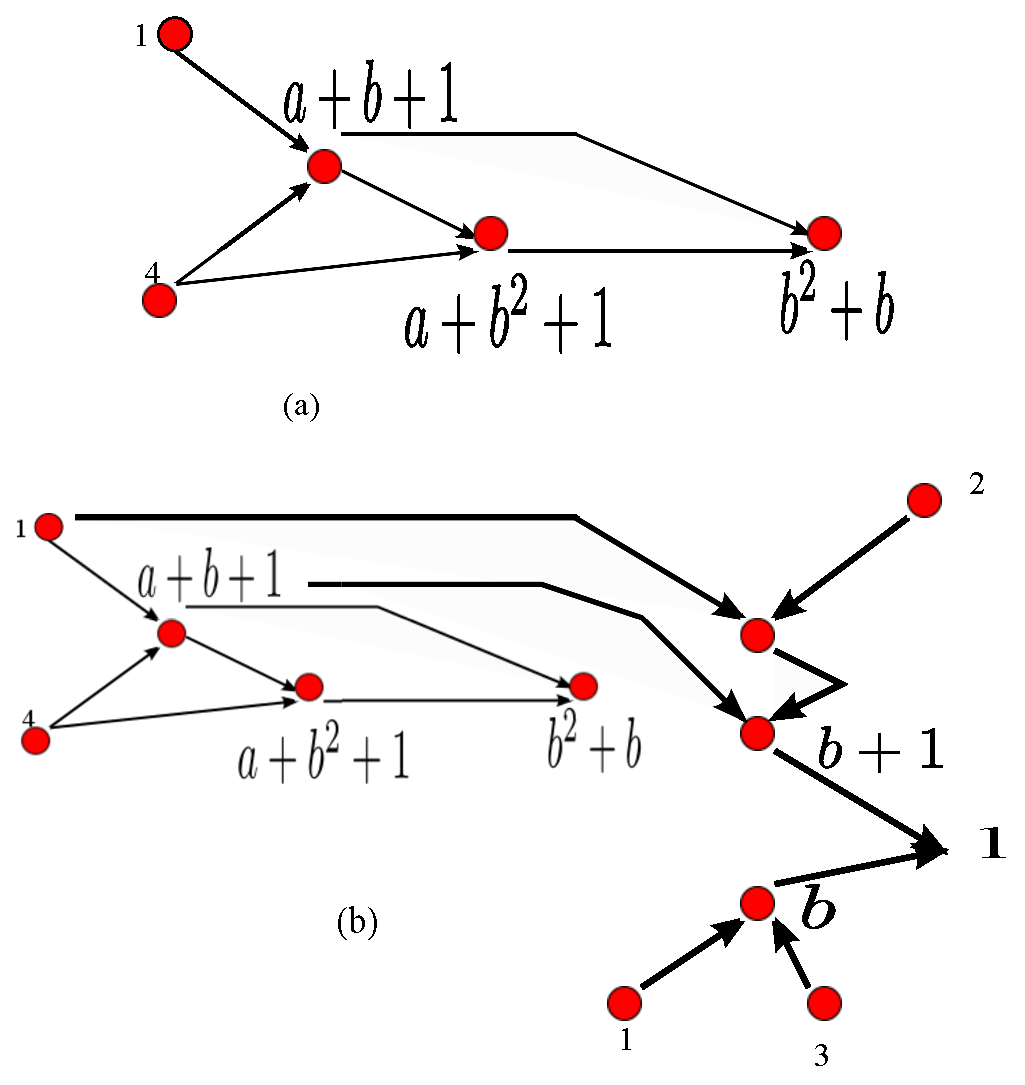
\includegraphics[scale=0.6]{trace.eps}
\caption{Keeping track of polynomials involved in $GB(J) = \{1\}$}
\label{fig:trace}
\end{figure}

Coming to the point: i) Keep track of all $Spoly(f_i,
f_j)\xrightarrow{f_1, \dots, f_s}_+ r$; ii) mark $f_i, f_j$ if $r\neq
0$; iii) Mark those $f_l$'s that have leading terms that cancel
monomial terms in $Spoly(f_i, f_j)$; iv) Build this Spoly graph (I
don't yet have a catchy name for this graph); v) Once $1\in J$ is
detected, traverse the graph to identify all the marked polynomials that were
used in obtaining this unit element. These polynomials constitute the
core.

\begin{Problem}
Does the approach guarantee a minimal core? If yes, how do we show it?
If not, we need to generate an example to understand it better. The
example that I have derived is too trivial. Probably we need to find
more complicated examples to test the idea. 
\end{Problem}

Questions and comments are welcome. 

%% Clauses:
%% \begin{align*}
%% \bar{a}\lor\bar{b}\\
%% a\lor\bar{b}\\
%% \bar{a}\lor b\\
%% a\lor b\\
%% x\lor y\\
%% y\lor z
%% \end{align*}


\section{Experiment results}
We have implemented our core extraction approach (the GB-Core
algorithm) using the \textsc{Singular} symbolic
algebra computation system [v. 3-1-6] \cite{DGPS}. With our
tool implementation, we have performed experiments to extract a
minimal unsat core from a given set of  
polynomials. Our experiments run on a desktop with
3.5GHz Intel $\text{Core}^\text{TM}$ i7-4770K Quad-core CPU, 16 GB RAM and
64-bit Ubuntu Linux OS.

%Nowadays most SAT benchmarks are huge, which choke our GB engine. 
Gr\"obner basis is not an efficient engine for solving contemporary
CNF-SAT benchmarks that are of large size. In order to validate our
approach, we use a customized  benchmark library: "aim-100" is revised
from ramdon 3-SAT benchmark "aim-50/100", "subset" series are generated for
random subset sum problems, "cocktail" is revised from a mixed
factorization/random 3-SAT benchmark, and "phole4/5" are generated by
adding redundandant clauses to pigeon hole benchmarks. Moreover, we
created SMPO/RH benchmarks that correspond to
equivalence checking instances of sequential Galois field normal basis
modulo multiplier implementations (also known as Agnew's multiplier \cite{SMPO}
and Reyhani-Hassan multiplier \cite{RHmulti} respectively) against the golden model spec. 
Similarly, the "MasVMon" benchmarks are the miter circuits of
 Mastrovito multipliers compared against  Montgomery
multipliers. The CNF formulae are translated as polynomial constraints
over $\mathbb{F}_2$ (as shown in \cite{condrat-tacas07}), and the
GB-Core algorithm is applied. 
%These benchmarks are in moderate size for our GB engine but not too trivial. 

\vspace{-0.1in}
\begin{table}[htb]
\centering
\caption{\centering Results of running benchmarks using our tool\\
\small{Asterisk($^*$) denotes a benchmark which is not converted from CNF benchmark}}
\begin{tabular}{|c||c|c|c|c|c|c|}
\hline
\multirow{4}{2.2cm}{\centering Benchmark} 
& \multirow{4}{0.9cm}{\centering \# Polys} 
& \multirow{4}{0.8cm}{\centering \# MUS} 
& \multirow{4}{1.9cm}{\centering Size of core w/ iterative refinement heuristic}
 & \multirow{4}{1.6cm}{\centering \# GB-core iterations}
 & \multirow{4}{2cm}{\centering \# Size of core after using syzygy heuristic}
 & \multirow{4}{1.3cm}{\centering Runtime (sec)} \\
  & & & & & & \\
    & & & & & & \\
      & & & & & & \\
\hline
\hline
$5\times 5$ SMPO & 240  & 137  & 137  & 8  &  & 3160\\
$4\times 4$ SMPO$^*$ & 84  & 21  & 21  & 1  &  & 125\\
$3\times 3$ SMPO$^*$ & 45  & 15  & 15  & 1  &  & 6.6\\
$3 \times 3$ SMPO & 17 & 2 & 2 & 1 &  & 0.07  \\
$4 \times 4$ MasVMont$^*$ & 148 & 83 & 83 & 1 &  & 23 \\
$3 \times 3$ MasVMont$^*$ & 84 & 53 & 53 & 1 &  & 4.3 \\
$2 \times 2$ MasVMont & 27 & 23 & 23 & 2 &  & 2.3 \\
$5\times 5$ RH$^*$ & 142  & 34  & 35  & 4  &  & 1001\\
$4\times 4$ RH$^*$ & 104  & 35  & 36  & 3  &  & 98\\
$3\times 3$ RH$^*$ & 50  & 20  & 20  & 1  &  & 2.9\\
aim-100 & 79 & 22 & 22 & 1  &  & 43\\
cocktail & 135 & 4 & 4 & 2 &  & 5 \\
subset-1 & 100 & 6 & 6 & 1 &  & 2.4 \\
subset-2 & 141 & 19 & 23 & 2 & 21 & 12 \\
subset-3 & 118 & 16 & 12 & 2 & 11 & 8.7 \\
phole4 & 104 & 10 & 16 & 1 & 10 & 4.4 \\
phole5 & 169 & 19 & 25 & 3 & 19 & 14 \\
\hline
\end{tabular}
\label{tab:result}  
\end{table} 

In Table \ref{tab:result}, we list the details of our experimental
results. In the table, \#Polys denotes the given number of polynomials
from which a core is to be extracted. \#MUS is the minimal core
extracted by PicoMUS. \#GB-core iterations corresponds to the
number of calling GB-core engine to arrive at an unsatisfiable core. The
second last column is showing the improvement of minimal core
size applying syzygy heuristic on cases which are not able to be
refined further with the iterative heuristic.
The data shows that in most of these
cases, our tool can produce a minimal core when our iterations
converge. From the experimental results we can also make the
observation that the GB-core algorithm, particularly Theorem
\ref{thm}, offers quite a lot of scope for identifying redundant
polynomials that can be eliminated from the core --- without resorting
to a brute-force membership check of every polynomial $f_i \in F -
\{f_i\}$. 




\section{Conclusions}
This paper addressed the problem of identifying an infeasible core of
a set of multivariate polynomials, with coefficients from a field,
that have no common zeros. The problem is posed in the context of
computational algebraic geometry and solved using the Gr\"obner basis
algorithm. We show that by recording the data produced by the
Buchberger's algorithm -- the $Spoly(f_i,f_j)$ pairs, as well as the
polynomials of $F$ used in the division process
$Spoly(f_i,f_j)\xrightarrow{F}_+ 1$ -- we can identify certain
conditions under which a polynomial can be discarded from a core. An
algorithm was implemented within the Singular computer algebra tool
and some experiments were conducted to validate the approach. While
the use of GB engines for SAT solving has a rich history, the problem
of unsat core identification hasn't been fully addressed by the SAT
community. We hope that this paper will kindle some interest in this
topic which is worthy of attention from the SAT community. 

%% \input{setup}
%% %\input{promodel}
%% %\input{solve}
%% \input{experiment_new}
%% \input{conclusion}
\section{Reduce the size of UNSAT core further}
In some
cases our iterative core refining algorithm cannot
give us the minimal core when it hits the fixpoint.
It indicates the limitation of using re-labelling 
strategy, therefore a new method to identify the 
redundancy in UNSAT core is needed.

The UNSAT core we obtained through our algorithm
is by nature a refutation polynomial that equals to 1:
$$1 = \sum_{i=1}^s c_i\cdot f_i$$
where $c_i \neq 0$ and $f_1,\dots,f_s$ form a core.
If by any means we find a relation between $f_k$ and set $\{f_j\}$
 ($f_k,f_j\in \{f_1,\dots,f_s\}$) and other polynomials
 in the core such that:
 $$f_k = \sum_{j\neq k} c_j'f_j$$
 Then we can substitute $f_k$ with other polynomials
 in the refutation polynomial. Thus, $f_k$ can be
 recognized as redundant polynomial in the core.
 
 Since coefficients $\{c_i\}$ are also polynomials in $\mathbb F[x_1,\dots,x_n]$, we can find 
 enormous number of combinations of $\{f_i\}$. Consider finding an algorithmic solution to 
 this problem without introducing extra search,
 we propose to utilize the \emph{syzygies} generated during
 executing the GB-core algorithm.
 
 In Buchberger's algorithm, if the polynomial division
 gives a nonzero remainder, then the information is 
 recorded. However, if the polynomial division results
 in a zero remainder nothing will be recorded. In order
 to gather more information from one iteration, we
 need to also record all quotients from s-polynomial
 reductions with 0 remainder. Those quotients (as well 
 as coefficients when pairing s-polynomials) form
 a syzygy:
\[
 \begin{cases}
 c_1^1f_1+c_2^1f_2+\cdots+c_s^1f_s = 0\\
 c_1^2f_1+c_2^2f_2+\cdots+c_s^2f_s  = 0\\
 \ \ \ \ \ \  \vdots \\
 c_1^mf_1+c_2^mf_2+\cdots+c_s^mf_s = 0  
 \end{cases}
\]
The matrix form of the syzygy is:
\begin{center}
\begin{align}
\label{mat:syzygy}
   \begin{bmatrix}
           c_1^1 & c_2^1 & \cdots & c_s^1 \\
           c_1^2 & c_2^2 & \cdots & c_s^2 \\
           \vdots & \vdots & \ddots & \vdots \\
           c_1^m & c_2^m & \cdots & c_s^m
         \end{bmatrix}
    \begin{bmatrix}
           f_{1} \\
           f_{2} \\
           \vdots \\
           f_{s}
         \end{bmatrix}
         &= 0
  \end{align}

\end{center}
 Here $\{f_1,f_2,\dots,f_s\}$ is the given core.
 Take one column of the syzygy matrix (e.g. $c_1^1, c_1^2, \dots, c_1^m$)
 and compute its minimal Gr\"obner basis. If the result is 1, then there exists some polynomial vector
 $r_1,r_2,\dots,r_m$ such that
 $$1 = r_1c_1^1 + r_2c_1^2 + \cdots + r_mc_1^m = \sum_{i=1}^m r_ic_1^i$$
 If we multiply the $i$-th row in above matrix with $r_i$ then add them up, 
 we get following equation
 \begin{center}
\begin{align}
   \begin{bmatrix}
           1 & \sum_{i=1}^m r_ic_2^i & \cdots & \sum_{i=1}^m r_ic_s^i
         \end{bmatrix}
    \begin{bmatrix}
           f_{1} \\
           f_{2} \\
           \vdots \\
           f_{s}
         \end{bmatrix}
         &= 0
  \end{align}

\end{center}
Which implies $f_1$ is a combination of $f_2,\dots,f_s$:
 $$f_1 = \sum_{i=1}^m r_ic_2^if_2 + \sum_{i=1}^m r_ic_3^if_3
 +\cdots + \sum_{i=1}^m r_ic_s^if_s$$
 Then we can remove $f_1$ from the core. By repeating
 this procedure, some redundant polynomials can be identified
 and size of UNSAT core will get closer to minimal.
 \begin{example}
 Assume we are given 9 polynomials from Example\ref{ex:1},
 execute GB-core algorithm and record syzygy. We
 write the coefficients as entries in following matrix:
 \[
 \begin{blockarray}{cccccccccccc}
  && f_1 & f_2 & f_3 & f_4 & f_5 & f_6 & f_7 & f_8 & f_9 & f_{10} \\
  \begin{block}{cc(cccccccccc)}
  Spoly(f_1,f_3)\ & & 1 & a+c+1 & b+1 &0&0&0&0&0&0&1\\
  Spoly(f_2,f_3)\ & & 0 & ac & b &0&0&0&0&0&0&0\\
  Spoly(f_1,f_4)\ & & 1 & c+1 & 1 &b&0&0&0&0&0&1\\
  Spoly(f_2,f_4)\ & & 0 & ac+a & 0 &b&0&0&0&0&0&0\\
  Spoly(f_1,f_5)\ & & 1 & a+c+1 & 0 &0&a&0&0&0&0&1\\
  \end{block}
  \end{blockarray}
 \]
 Usually we will get extra columns comparing to syzygy matrix in (\ref{mat:syzygy}).
 In this example we add an extra column for coefficient of $f_{10}$
 since some s-polynomial pairs require new generator $f_{10}$
 as divisor during reduction. In order to remove this
 extra column, we need to turn nonzero entries in this column
 to 0 through matrix manipulations. Recall that
 we record $f_{10}$ as nonzero remainder when reducing s-polynomial
 pair $Spoly(f_1,f_2)$, we extract corresponding submatrix from the coefficient matrix $M$
 $$(1 ac+a+c+1 1 0 0 0 0 0 0 )$$
 It represents $f_{10}$ is a combination of $f_1$ to $f_9$:
 $$f_{10} = f_1 + (ac+a+c+1)f_2 + f_3$$
 It can be written in matrix with column $f_{10}$ as follows:
  \[
 \begin{blockarray}{cccccccccccc}
  && f_1 & f_2 & f_3 & f_4 & f_5 & f_6 & f_7 & f_8 & f_9 & f_{10} \\
  \begin{block}{cc(cccccccccc)}
  Spoly(f_1,f_2)& & 1 & ac+a+c+1 & 1 &0&0&0&0&0&0&1\\
  \end{block}
  \end{blockarray}
 \]
 By adding this row to corresponding rows in the matrix,
 we can get syzygy matrix only for polynomials
 in the core:
  \[
 \begin{blockarray}{ccccccccccc}
  && f_1 & f_2 & f_3 & f_4 & f_5 & f_6 & f_7 & f_8 & f_9  \\
  \begin{block}{cc(ccccccccc)}
  Spoly(f_1,f_3)\ & & 0 & ac & b &0&0&0&0&0&0\\
  Spoly(f_2,f_3)\  && 0 & ac & b &0&0&0&0&0&0\\
  Spoly(f_1,f_4)\  && 0 & ac+a & 0 &b&0&0&0&0&0\\
  Spoly(f_2,f_4)\  && 0 & ac+a & 0 &b&0&0&0&0&0\\
  Spoly(f_1,f_5)\  && 0 & ac & 1 &0&a&0&0&0&0\\
  \end{block}
  \end{blockarray}
 \]
 We find out there is a ``1" entry in column $f_3$, so 
 its minimal GB equals to 1. Therefore $f_3$ can be
 recognized as redundant polynomial and removed from the UNSAT core. 
 
 \end{example}



%%%%%%%%%%%%%%%%%%%% The bibliography %%%%%%%%%%%%%%%%%%%%%%%%%%%%
%\bibliographystyle{splncs03}
\bibliographystyle{IEEEtran}
%\bibliography{cf}
\bibliography{tim,logic,oldlogic,cnfsat}
\end{document} 




